% make_report (ai/skills/make_report). Компиляция: tectonic report.tex
\documentclass[11pt,a4paper]{article}

\usepackage{fontspec}
\usepackage{polyglossia}
\setmainlanguage{russian}
\setotherlanguage{english}
\setmainfont{Times New Roman}
\newfontfamily\cyrillicfont{Times New Roman}
\setsansfont{Helvetica}
\newfontfamily\cyrillicfontsf{Helvetica}
\setmonofont{Menlo}[Scale=0.85]
\newfontfamily\cyrillicfonttt{Menlo}[Scale=0.85]

\usepackage[margin=2cm]{geometry}
\usepackage{amsmath,amssymb}
\usepackage{booktabs,array,multirow,tabularx}
\usepackage{graphicx}
\usepackage{float}
\usepackage[font=small,labelsep=period]{caption}
\usepackage[shortlabels]{enumitem}
\usepackage{xcolor}
\usepackage{tikz}
\usetikzlibrary{arrows.meta}
\usepackage[colorlinks=true,linkcolor=black,urlcolor=blue!50!black,citecolor=black]{hyperref}

\setlist{nosep,leftmargin=1.2em}
\setlength{\parindent}{0pt}
\setlength{\parskip}{4pt}
\setlength{\emergencystretch}{3em}
\sloppy
\graphicspath{{figures/}}

\definecolor{ml}{HTML}{2A78D6}
\definecolor{ppub}{HTML}{EB6834}
\definecolor{pfree}{HTML}{1BAF7A}
\definecolor{poff}{HTML}{EDA100}

\newcommand{\NMAD}{\mathrm{NMAD}}
\newcommand{\fnref}[1]{\textsuperscript{\ref{#1}}}
\newcolumntype{Y}{>{\raggedright\arraybackslash}X}

\title{Отчёт за 6 ноября 2026}
\author{}
\date{}

\begin{document}
\maketitle

\section{Сетап эксперимента}

\subsection{Данные}

Источник — каталог и мозаики Euclid Q1 MER.

\textbf{Изображение} — тензор $12\times64\times64$ ($6.4''\times6.4''$, объект в центре):
\begin{itemize}
  \item слои 0–3 — поток в четырёх полосах Euclid, каждая — отдельный одноцветный слой (не RGB): VIS — одна широкая оптическая полоса, $\approx0.55$–$0.9$ мкм; Y, J, H — ближний ИК, $\approx0.95$–$2.0$ мкм;
  \item слои 4–7 — ошибка потока; 8–11 — маска (1 — годный пиксель; плохие пиксели в слоях 0–7 обнулены);
  \item «VIS» на графиках — звёздная величина объекта в полосе VIS (AB): чем больше число, тем объект тусклее.
\end{itemize}

\textbf{Таблица} — тензор $14\times2$ (14 полос $\times$ поток и ошибка), маска наличия полос (14) и описание фильтров $14\times18$:
\begin{itemize}
  \item полосы: Euclid VIS, Y, J, H; UNIONS $ugriz$ (поле N); DECam $ugriz$ (поля F/S). Наземная фотометрия F/S переводится в полосы UNIONS (ниже), чтобы обучение и тест были в одной системе фильтров;
  \item поток апертурный: свет суммируется в круге размером $2\times$FWHM (FWHM — ширина изображения звезды на половине яркости). Круг одинаков во всех полосах, поэтому цвета сравнимы; так же считает официальный PHZ\footnote{\label{fn:tucci}Tucci et al. (Euclid Collaboration), 2026, A\&A, 711, A5; arXiv:2503.15306.};
  \item описание фильтра — 18 чисел из его публичной кривой пропускания, одинаковых для всех объектов: логарифм эффективной (pivot) длины волны, логарифм ширины и доли пропускания в 16 логарифмических интервалах 0.3–2.1 мкм. Так модель узнаёт полосу по её положению в спектре, а не по номеру столбца;
  \item морфологии в таблице нет — её несут изображения.
\end{itemize}

\textbf{Перевод фотометрии F/S в полосы N (UNIONS).} Фильтры DECam и UNIONS разные. В проверочном прогоне без перевода (тот же рецепт) модель, обученная на DECam, давала на DESI в поле N NMAD 0.057 вместо 0.026.
\begin{itemize}
  \item Для объекта F/S подбирается шаблон спектра (31 шаблон COSMOS с эмиссионными линиями) при фото-$z$ Phosphoros юга; по шаблону считаются потоки через публичные кривые фильтров UNIONS.
  \item Полоса $u$: шаблонный поток плюс шум по опубликованной глубине CFIS ($5\sigma=24.2$ AB).
  \item Нуль-пункты (поправочные множители к потоку в каждом фильтре, калибровка) Euclid подобраны только по меткам F, UNIONS равны 1. Данные N не используются.
  \item Около 2\% строк обучения (SDSS и объекты с неудачным фитом) остаются в полосах DECam.
\end{itemize}

\textbf{Спектр} — бесщелевой спектр NISP; есть у части объектов F/S; только в предобучении.

\textbf{Подготовка чисел} (для изображений и таблицы одинаково):
\begin{itemize}
  \item поток $f$ ($\mu$Jy) $\to\operatorname{asinh}(f/s)$, $s$ — медиана потока в полосе по трейну. Сжимает диапазон как логарифм, но определена при $f\le0$ (шум): около нуля $\approx f/s$, при больших $f$ $\approx\ln(2f/s)$ — asinh-величины\footnote{\label{fn:lupton}Lupton et al., 1999, AJ, 118, 1406.};
  \item ошибка $\sigma\to\log(1+\sigma/s)$;
  \item затем каждый слой стандартизуется: среднее 0, разброс 1 по трейну.
\end{itemize}

\begin{table}[H]
\centering\small
\caption{Объём выборок.}
\begin{tabular}{lrrrr}
\toprule
Этап & F & S & N & Всего \\
\midrule
Предобучение CLIP, без меток & 591\,834 & 589\,330 & 0 & 1\,181\,164 \\
Дообучение: метки & 20\,778 & 378 & 0 & 21\,156 \\
Валидация & 1\,062 & 9 & 0 & 1\,071 \\
Тест: DESI, NEP-Wide, HETDEX & 0 & 0 & 53\,620 & 53\,620 \\
\bottomrule
\end{tabular}
\end{table}

\begin{table}[H]
\centering\small
\caption{Обзор меток. «Флаг» — оценка надёжности $z$ в самом обзоре (4 — самая высокая).}
\begin{tabular}{>{\raggedright\arraybackslash}p{6.4cm}l>{\raggedright\arraybackslash}p{4.4cm}l}
\toprule
Обзор & Поле & Число & Роль \\
\midrule
PRIMUS, флаг 4 & F & 10\,205 & обучение \\
OzDES DR2 & F & 5\,065 & обучение \\
OzDES, флаг 3 & F & 1\,721 & обучение \\
ACES, флаг 4 & F & 1\,004 & обучение \\
VANDELS DR4 (CDFS) & F & 374 & обучение \\
GOODS, VLT/VIMOS, низкое / среднее разрешение & F & 241 / 164 & обучение \\
GOODS, VLT/FORS2 & F & 136 & обучение \\
3D-HST (Hubble, CDFS): обычные спектры / бесщелевые спектры Hubble, только точные — 68\%-интервал $z$ уже 2\% от $(1+z)$ & F & 580 / 1\,550 & обучение \\
MUSE (эмиссионные / яркие) + SDSS & F & 666 / 64 + 92 (в обучении 800) & обучение \\
SDSS & S & 387 & обучение \\
DESI DR1 + 23 SDSS & N & 40\,013 & тест \\
NEP-Wide\fnref{fn:kim} & N & 748 & тест \\
HETDEX HPSC2\fnref{fn:hpsc}, [OII] & N & 12\,859 & тест \\
\bottomrule
\end{tabular}
\end{table}
Источники меток: NEP-Wide\footnote{\label{fn:kim}Kim et al., 2025, ApJS, 277, 41.}, HETDEX HPSC2\footnote{\label{fn:hpsc}Mentuch Cooper et al., 2026, ApJS; arXiv:2606.04208. Каталог: Zenodo, doi:10.5281/zenodo.19581262.}.

\begin{figure}[H]
\centering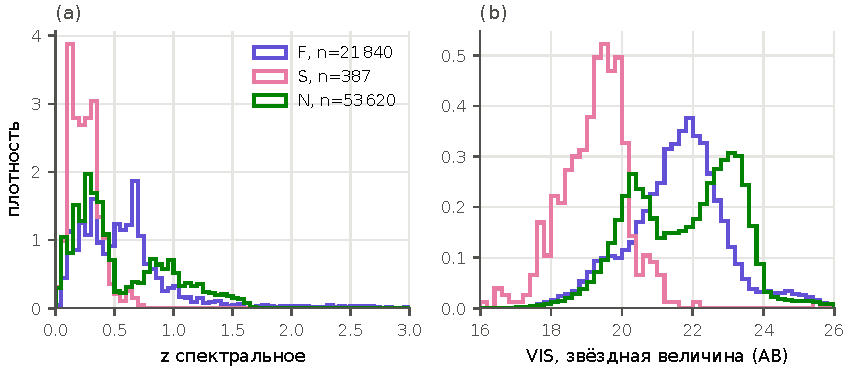
\includegraphics[width=\linewidth]{fig_dist.pdf}
\caption{}
\label{fig:dist}
\end{figure}

\subsection{Трейн-выборка (поля F и S)}

\begin{table}[H]
\centering\small
\caption{Метки обучения и валидации (поля F и S).}
\begin{tabularx}{\linewidth}{lrY}
\toprule
Набор & $n$ & Состав \\
\midrule
F, 39 тайлов & 17\,809 & PRIMUS, OzDES, ACES, VANDELS, GOODS \\
F, ещё 10 тайлов & 1\,101 & OzDES \\
CDFS (3D-HST) & 2\,130 & 580 обычных спектров, 1\,550 бесщелевых спектров Hubble \\
MUSE + SDSS & 800 & без пересечений с другими наборами \\
SDSS, поле S & 387 & — \\
\midrule
Все метки F и S & 22\,227 & обучение 21\,156, валидация 1\,071 \\
Немеченые F/S & 1\,181\,164 & изображения, таблицы, спектры — предобучение CLIP \\
\bottomrule
\end{tabularx}
\end{table}
\begin{itemize}
  \item \textbf{Поля F и S} используются для обучения целиком: все объекты без меток — в предобучении CLIP, все метки (F и 387 SDSS в S) — в дообучении и валидации.
  \item \textbf{Поле N в обучении не используется:} ни метки, ни фотометрия, ни изображения, ни нуль-пункты.
  \item \textbf{Валидация} — 1\,071 метка из всех меток F и S: 12 интервалов по $\log(1+z)$ на $0<z<3$, по 125 объектов в интервале; при $z>1.25$ меток мало, поэтому берём 15\% интервала (24–61 объект), чтобы не обеднять обучение. По ней смотрим NMAD по эпохам; ранней остановки и подбора гиперпараметров по ней нет.
\end{itemize}

\subsection{Тест-выборка (поле N)}

\begin{table}[H]
\centering\small
\caption{Тестовые наборы.}
\begin{tabular}{lrl}
\toprule
Набор & $n$ & Источник \\
\midrule
DESI & 40\,013 & DESI DR1 + 23 SDSS \\
NEP-Wide & 748 & NEP-Wide\fnref{fn:kim} \\
HETDEX & 12\,859 & HPSC2\fnref{fn:hpsc} \\
\bottomrule
\end{tabular}
\end{table}

\subsection{Модели}

\begin{figure}[H]
\centering
\begin{tikzpicture}[font=\sffamily\scriptsize,
  box/.style={draw=black!40, rounded corners=2pt, align=center, inner sep=3pt, minimum height=9mm, text width=30mm, fill=black!3, execute at begin node={\hyphenpenalty=10000\exhyphenpenalty=10000}},
  wide/.style={box, text width=40mm},
  enc/.style={box, fill=ml!8, draw=ml!70},
  arr/.style={-{Stealth[length=1.7mm]}, draw=black!55}]
\node[anchor=west, font=\sffamily\small\bfseries] at (-1.45,0.85) {(a) Предобучение CLIP: 1.18 млн объектов F/S без меток; батч 256, 12 эпох, 2 сида};
\node[box] (im) at (0,0) {изображение\\$12\times64\times64$};
\node[box] (tb) at (0,-1.3) {таблица: токен на полосу\\(поток, ошибка, фильтр)};
\node[box] (sp) at (0,-2.6) {спектр NISP\\(часть объектов)};
\node[enc] (ei) at (3.85,0) {CNN, ResNet-18-подобная;\\2.80 млн $\to$ 256};
\node[enc] (et) at (3.85,-1.3) {Transformer, 2 слоя;\\0.32 млн $\to$ 256};
\node[enc] (es) at (3.85,-2.6) {энкодер спектров\\$\to$ 256};
\node[box] (pr) at (7.7,-1.3) {2 полносвязных слоя\\$256\to256\to128$\\(своя пара на вход),\\нормировка вектора};
\node[wide] (lo) at (11.85,-1.3) {InfoNCE, $T=0.1$:\\косинус между векторами\\своего объекта больше,\\чем с чужими};
\foreach \a/\b in {im/ei, tb/et, sp/es, pr/lo} \draw[arr] (\a) -- (\b);
\foreach \a in {ei, et, es} \draw[arr] (\a.east) -- (pr.west);
\node[anchor=west, font=\sffamily\small\bfseries] at (-1.45,-3.65) {(b) Дообучение всей сети: 21\,156 меток F и S; батч 128, 40 эпох, 6 сидов};
\node[box] (im2) at (0,-4.5) {изображение};
\node[box] (tb2) at (0,-5.8) {таблица};
\node[enc] (ei2) at (3.85,-4.5) {CNN из (a) $\to$ 256};
\node[enc] (et2) at (3.85,-5.8) {Transformer из (a) $\to$ 256};
\node[box] (ct) at (7.7,-5.15) {склейка\\256 + 256 + 2 флага\\наличия = 514};
\node[wide] (mlp) at (11.85,-5.15) {MLP $514{\to}256{\to}128{\to}200$\\softmax по 200 бинам $\log(1{+}z)$\\лосс: кросс-энтропия,\\веса объектов $\propto p(z)^{-0.5}$};
\foreach \a/\b in {im2/ei2, tb2/et2, ct/mlp} \draw[arr] (\a) -- (\b);
\foreach \a in {ei2, et2} \draw[arr] (\a.east) -- (ct.west);
\end{tikzpicture}
\caption{}
\end{figure}

\textbf{Устройство.} Полносвязные слои $256\to256\to128$ и нормировка нужны только в предобучении: они переводят выходы энкодеров в общее пространство, где сравниваются векторы разных входов; при дообучении они отбрасываются. Энкодер изображений: свёртка $3\times3$ ($12\to32$ канала), 4 стадии шириной 32/64/128/256 по 2 остаточных блока, GroupNorm (8 групп), ReLU, среднее по пикселям. Энкодер таблицы: токен полосы — 2 числа + 18 чисел описания фильтра $\to$ MLP 128; Transformer $d=128$, 4 головы, FFN 256, GELU; среднее по измеренным полосам.

\textbf{Общее:} AdamW, шаг $3\cdot10^{-4}$, затухание весов $10^{-4}$; шаг растёт линейно 5 эпох, затем убывает по косинусу; норма градиента обрезается до 5; аугментация — повороты на $90^\circ$ и отражения.

\textbf{Прогноз:} $z$ — медиана распределения $p(z)$ по 200 бинам; итог — среднее $z$ по 6 сидам.


\textbf{Методы сравнения:}
\begin{itemize}
  \item \textbf{Phosphoros} — подбор шаблонов спектров, не обучается: для каждого $z$ на сетке 0–6 и каждого из 31 шаблона COSMOS (с эмиссионными линиями и пылью) считается $\chi^2$ с измеренными потоками. Наш перезапуск публичной версии 2.2.1 с официальными настройками и нуль-пунктами Euclid\fnref{fn:tucci}. Нуль-пункты UNIONS подобраны в том числе по спектрам DESI в поле N — информация из тестового поля, которой у нашей модели нет.
  \item \textbf{PHZ Euclid} — официальный каталог фото-$z$ Euclid Q1 (тот же Phosphoros в конвейере Euclid).
  \item \textbf{Классический ML} — CatBoost, Random Forest, ANNz, LLR ($k$-NN), GAM на тех же 21\,156 строках и табличных признаках (Euclid и UNIONS, без изображений); гиперпараметры фиксированы заранее.
\end{itemize}

\subsection{Обучение}

Сходимость — на рис.~\ref{fig:train}: (a) лосс InfoNCE предобучения, (b) кросс-энтропия дообучения, (c) NMAD на валидации; горизонтали — Phosphoros и PHZ Euclid на тех же объектах. Ранней остановки нет. Железо — NVIDIA RTX A6000 48 ГБ.

\begin{figure}[H]
\centering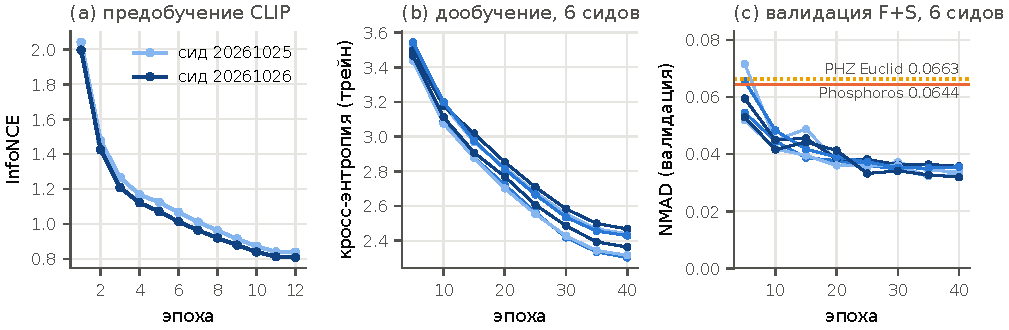
\includegraphics[width=\linewidth]{fig_train.pdf}
\caption{}
\label{fig:train}
\end{figure}

\section{Результаты эксперимента}


\subsection{Метрики}

\begin{table}[H]
\centering\small
\caption{NMAD / доля выбросов. $n$ — объекты, для которых есть прогнозы всех методов.}
\resizebox{\linewidth}{!}{%
\begin{tabular}{lrccc}
\toprule
Набор & $n$ & \textcolor{ml}{Наша модель} & \textcolor{ppub}{Phosphoros} & PHZ Euclid \\
\midrule
\csname @@input\endcsname tables/metrics.tex 
\bottomrule
\end{tabular}%
}
\end{table}

\begin{table}[H]
\centering\small
\caption{$\Delta\NMAD$ = наша модель $-$ метод сравнения, 95\% ДИ (тайловый бутстрэп, $B=2000$); $<0$ — наша модель лучше.}
\resizebox{\linewidth}{!}{%
\begin{tabular}{lcc}
\toprule
Набор & против Phosphoros & против PHZ Euclid \\
\midrule
\csname @@input\endcsname tables/metrics_delta.tex 
\bottomrule
\end{tabular}%
}
\end{table}

\begin{table}[H]
\centering\small
\caption{Бейзлайны. NMAD / выбросы; последний столбец — $\Delta\NMAD$ = наша модель $-$ метод на «N, все источники», 95\% ДИ. Классический ML — на тех же строках и табличных признаках, что у нашей модели, без изображений.}
\resizebox{\linewidth}{!}{%
\begin{tabular}{lccccc}
\toprule
Метод & N, все & N: DESI & N: NEP-Wide & N: HETDEX & $\Delta\NMAD$ \\
\midrule
\csname @@input\endcsname tables/classical.tex 
\bottomrule
\end{tabular}%
}
\end{table}

\begin{figure}[H]
\centering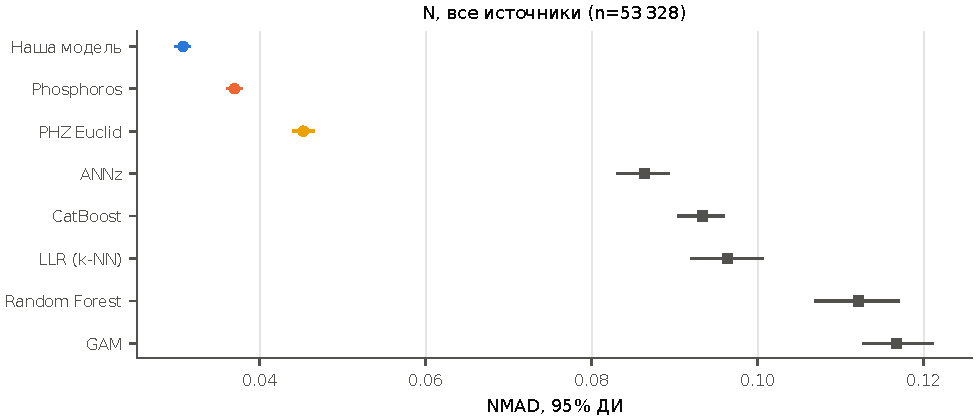
\includegraphics[width=\linewidth]{fig_baselines.pdf}
\caption{}
\end{figure}


\subsection{Графики}

\begin{figure}[H]
\centering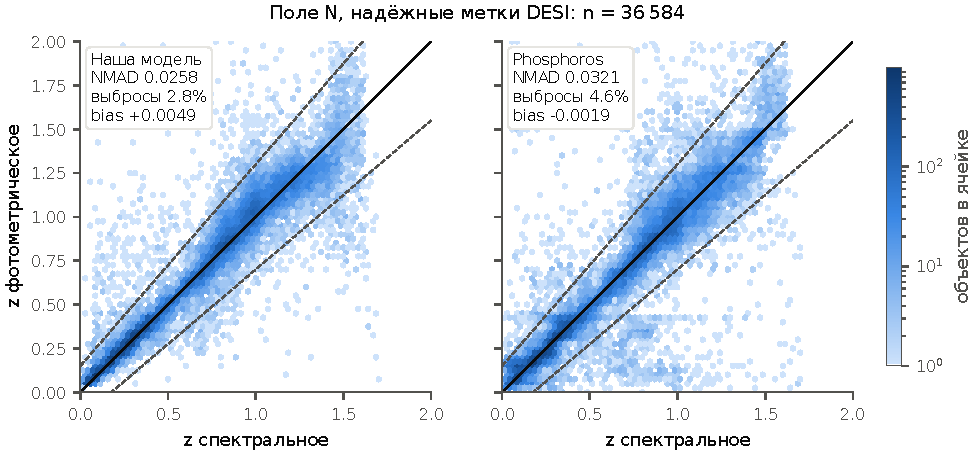
\includegraphics[width=\linewidth]{fig_scatter_N.pdf}
\caption{}
\end{figure}

\begin{figure}[H]
\centering\IfFileExists{figures/fig_scatter_Nall.pdf}{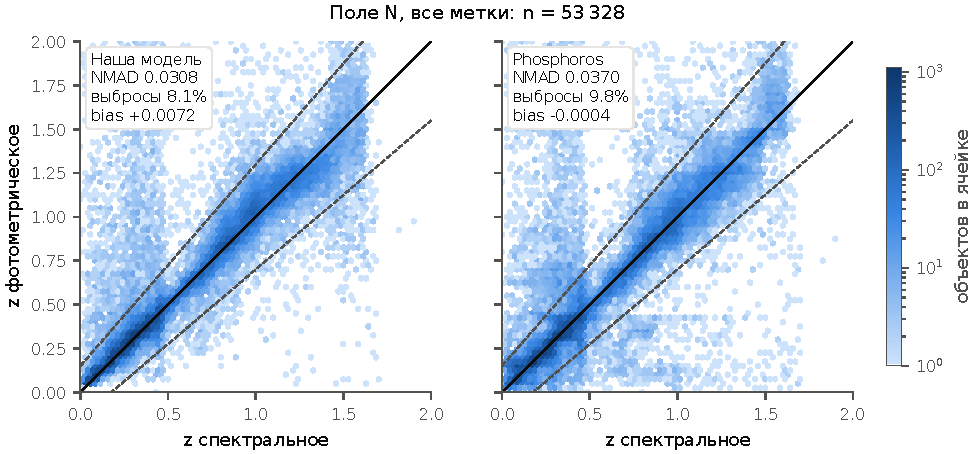
\includegraphics[width=\linewidth]{fig_scatter_Nall.pdf}}{\fbox{\parbox{0.9\linewidth}{\centering график появится после пересчёта финальной модели}}}
\caption{}
\end{figure}

\begin{figure}[H]
\centering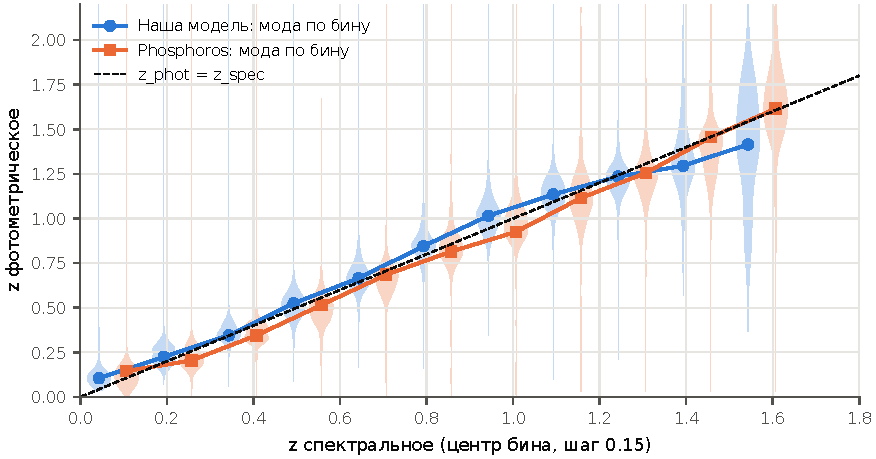
\includegraphics[width=\linewidth]{fig_modes.pdf}
\caption{}
\label{fig:modes}
\end{figure}

\begin{figure}[H]
\centering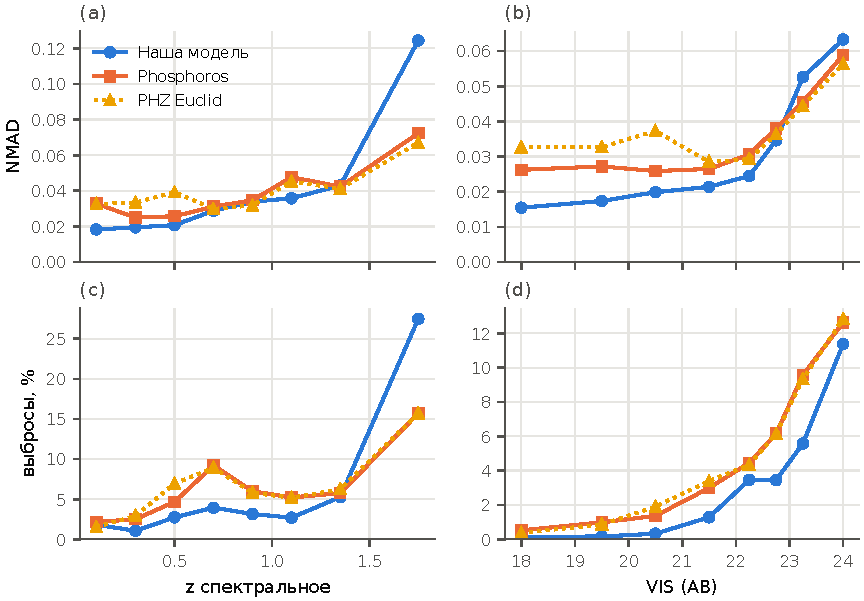
\includegraphics[width=\linewidth]{fig_bins.pdf}
\caption{}
\label{fig:bins}
\end{figure}
\begin{itemize}
  \item Рис.~\ref{fig:modes} и~\ref{fig:bins} — надёжные метки DESI ($n=36\,584$).
  \item По $z$: NMAD нашей модели ниже, чем у Phosphoros и PHZ Euclid, при $z<0.8$ и $1.0\le z<1.2$; при $0.8\le z<1.0$ и $1.2\le z<1.5$ — на их уровне.
  \item По яркости: NMAD ниже всех при VIS $<23$; у самых тусклых (VIS $>23$) — хуже: 0.053–0.063 против 0.044–0.059. Доля выбросов меньше во всех интервалах VIS.
  \item Слабое место — $1.5\le z<2.0$: NMAD 0.124 и 27.5\% выбросов против 0.067–0.072 и 15.7\% у Phosphoros и PHZ Euclid.
\end{itemize}


\end{document}
